   
  \chapter{Teorie a technologie}
  V této části si přiblížíme technologie potřebné k návrhu a vývoji webové služby specifikované v zadání práce. Postupně budou vysvětleny všechny zásadní pojmy, které pomůžou čtenáři doplnit znalosti.
  
  
  % ukazka citace
  \section{REST}
	Representational state transfer (dále jen REST) je architektura pro komunikaci \cite{rest} mezi distribuovanými systémy. Aby se rozhraní mohlo nazývat REST musí splňovat těchto 5 omezení/principů \cite{restThesis}: 
	\begin{itemize}
		\item Klient-Server(Clien-Server) - Toto omezení staví na principu oddělení zodpovědností (Separation of Concerns), nebo-li je klientská část starající se o uživatelské rozhraní a serverová část přistupující k databázi. Zlepšuje škálovatelnost sytému a zjednodušuje použitelnost na různých platformách.
		\item Bezestavovost(Stateless) - Každý požadavek musí přenášet všechna související data, server totiž neuchovává žádné informace o nynějším spojením a každý požadavek bere jako nový.
		\item Keš(Cache) - Data přenášená v odpovědi mohou být označená jako kešovatelná, tudíž si je klient může uložit a kdykoliv použít znova.
		\item Jednotné rozhraní(Unified interface) - Základem tohoto omezení je princip HATEOAS (Hypermedia As The Engine Of Application State), které říká, že klient nepotřebuje znát pravidla komunikace dopředu a data musí obsahovat odkazy na další data v aplikaci. Jasně definovaná adresa zdroje (např. URI), reprezentace přenášených dat (např. HTML), typ média (např. JSON)
		\item Vrstvený systém(Layered system) - Přidáním vrstev se aplikace, kde každá vrstva je izolovaná a může komunikovat jenom s následující vrstvou, zpřehlední a zlepší se škálovatelnost.
	\end{itemize}
	Těchto 5 základních pravidel by mělo být dodrženo, aby se aplikace mohla nazývat RESTful.  
	
	Nejčastějším typem protokolu využívající tuto architekturu je Hypertext Transfer Protocol(HTTP). Pomocí třech hlavních metod GET, POST, DELETE v požadavku poslaného z klienta server buď odpovídajíce vrátí požadovaná data, přijme data poslané v těle a například uloží do databáze nebo vymaže data. 
  
  
 \section{LaTeX}
	Vychází z typografického sázecího systému TeX, který takto popisuje Pavel Satrapa ve své knize \cite{latex}: \enquote{\textit{Patří do rodiny tak zvaných značkovacích jazyků (markup languages) a dal by se zjednodušeně charakterizovat jako programovací jazyk pro sazbu textů. Jeho základním vstupem je textový soubor, který obsahuje jak sázený dokument, tak příkazy ovlivňující sazbu. Určité znaky mají přiřazen speciální význam a jejich prostřednictvím jsou v textu odlišeny řídicí konstrukce. Typickým příkladem je zpětné lomítko, jímž začínají příkazy.}}
	 
	LaTex je rozšíření TeXu o balíček přednastavených řídících konstrukcí. Hlavní cílem těchto systému je jednoduchost pro psaní matematických a jiných vzorců. Ovšem je také velmi oblíben kvůli silné možnosti upravovat dokumenty ke svému zalibení.
	
	Příkazy a text se píše do souborů s příponou tex tyto soubory musí dodržovat jistou stromovou strukturou. V kořenu stromu je jeden hlavní soubor, do kterého jsou vnořovány další. To napomáhá přehlednosti velkých dokumentů a také používání již vytvořených. Následně se musí všechny soubory zkompilovat.Výstupním souborem můžou být ruzné formáty např. PDF, DVI aj. 

\section{Java EE}
	Tato platforma je rozšířením standardní Javy SE a je primárně určená pro vývoj webových aplikací. Java EE potřebuje ke svému fungování aplikační server, který se stará o požadavky, komunikuje s databází apod. Hlavním výstupem aplikace je HTML generované na serveru a zpracované na klientovi, to je rozdíl oproti standardní Javě, kde vše probíhá na klientovi. 

\section{PDF}
	Portable Document Format(dále jen PDF), jak už název napovídá jedná se o formát dokumentů, jejichž hlavním cílem je poskytování nazávislosti na platformě. Soubor se skládá ze čtyř komponent: 
	\begin{itemize}
		\item Objekty(Objects) - Základní jednotka celého souboru např. Pole, Čísla, Řetězce znaků. Jednotlivé objekty se popisují množinou znaků, která je definována lexikálními konvencemi.
		\item Struktura objektů(File Structure) - Soubor je rozdělen na čtyři části: 
			\begin{figure}
				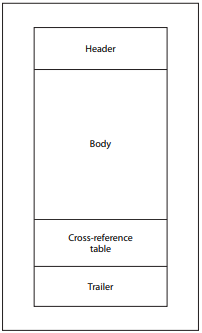
\includegraphics[scale=0.8]{Untitled}
				\centering
				\caption{Struktura objektů}
			\end{figure}
			\begin{itemize}
				\item hlavička - identifikuje verzi PDF
				\item tělo - obsahuje použité objekty, které reprezentují obsah dokumentu
				\item tabulka odkazů - obsahuje odkazy na objekty v podobě počtu bytů od začátku souboru, kvůli náhodnému přístupu bez potřeby číst celý soubor
				\item závěrečná sekce - udává pozici tabulky odkazů a speciálních objektů
			\end{itemize}
		\item Struktura dokumentu(Document Structure) - Popisuje hierarchickou strukturu objektů v těle dokumentu.
		\item Content stream - Objekt v kterém se nacházejí instrukce k vykreslování grafických elementů. 
	\end{itemize}
	

\section{FURPS+}
	Vzniklo rozšířením klasifikací požadavků FURPS(\textbf{F}unctionality, \textbf{U}sability, \textbf{R}eliability, \textbf{P}erformance, \textbf{S}upportability) s kterou přišel Robert Grady v roce 1992. Znaménko "+" ve zkratce přidává požadavky a omezení na design, implementaci, rozhraní a hardware. 
	
	\begin{itemize}
		\item Funkční požadavky
			\begin{itemize}
				\item Functionality - Požadavky popisujicí všechny hlavní prvky produktu i důležité aspekty z pohledu architektury např. lokalizovaný systém pro více jazyků.
			\end{itemize}
		\item Nefunknční požadavky
			\begin{itemize}
				\item Usability - Zaměřuje se na uživatelskou přívětivost nejenom samotné aplikace, ale i dokumentace apod., týkající se estetiky a konzistence
				\item Reliability - Spolehlivost systému v podobě času fungování, správnosti fungování a četnosti výpadků
				\item Performance - Vypovídá o výkonnosti systému, jak rychle dokáže zpracovávat požadavky, nastartovat atd.
				\item Supportability - Popisuje testovatelnost, škálovatelnost, konfigurovatelnost...
				\item Design - Omezení na design systému např. požadavek na relační databázi
				\item Implementation - Specifikuje typ prorgamovacího jazyku, platformu apod.
				\item Interface - Komununikace s externímy systémy
				\item Physical - Definuje požadavky na hardware, na kterém daný software poběží i co se týče velikosti
			\end{itemize}
	\end{itemize}
	
	Toto rozdělení nám pomáhá identifikovat požadavky. Přispívá k vyšší kvalitě systému a snižuje pravděpodobnost přehlédnutí funkcionality.